\documentclass[tikz,border=0pt]{standalone}
% rppreamble.tex -- engine switch for the standalone figure builds.
% Tectonic/XeTeX loads xeCJK; pdfLaTeX (arXiv) loads CJKutf8 with gbsn.
% Every Chinese string goes through \zh{...}. main.tex repeats this switch,
% and the standalone package skips this preamble when main.tex inputs a figure.
\usepackage{iftex}
\ifXeTeX
  \usepackage{xeCJK}
  \setCJKmainfont{FandolSong-Regular.otf}
  \setCJKsansfont{FandolHei-Regular.otf}
  \setCJKmonofont{FandolHei-Regular.otf}
  \providecommand{\zh}[1]{#1}
\else
  \usepackage[T1]{fontenc}
  \usepackage[utf8]{inputenc}
  \usepackage{lmodern}
  \usepackage{CJKutf8}
  \DeclareRobustCommand{\zh}[1]{\begin{CJK}{UTF8}{gbsn}#1\end{CJK}}
\fi
\usepackage{amsmath,amssymb}
\usepackage{xcolor}
\usepackage{tikz}
% rpstyle.tex -- the one visual system shared by every ReadProof figure.
% Loaded by each standalone figure (through rppreamble.tex) and by main.tex.
% Palette: ink #03080a for text and plain flow; violet #5b4be8 for ReadProof
% components; red #e2452a for walls and failures; greys for neutral parts.
% Labels are set at 8--8.5 pt so they stay readable at 100% in the paper.
\usetikzlibrary{positioning,arrows.meta,calc,shapes.geometric,shapes.misc,fit,backgrounds}
\definecolor{rpInk}{HTML}{03080A}
\definecolor{rpViolet}{HTML}{5B4BE8}
\definecolor{rpRed}{HTML}{E2452A}
\definecolor{rpGrey}{HTML}{8C929B}
\definecolor{rpGreyDark}{HTML}{50565E}
\definecolor{rpGreyFill}{HTML}{F2F3F5}
\definecolor{rpVioletFill}{HTML}{ECE9FC}
\definecolor{rpVioletPale}{HTML}{F8F7FE}
\definecolor{rpRedFill}{HTML}{FCE9E5}
\providecommand{\rpfont}{\fontsize{8.5}{10}\selectfont\sffamily}
\providecommand{\rpsmall}{\fontsize{8}{9.4}\selectfont\sffamily}
\providecommand{\rpmono}{\fontsize{7.8}{9.2}\selectfont\ttfamily}
\providecommand{\rpdot}{\,\ensuremath{\cdot}\,}
\providecommand{\rpto}{\ensuremath{\rightarrow}}
\providecommand{\rpt}[1]{{\fontsize{8.5}{10.2}\selectfont\bfseries #1}}% node title
\tikzset{
  rp base/.style={rounded corners=3pt, line width=0.6pt, align=center,
    inner xsep=4pt, inner ysep=2.6pt, font=\rpsmall, text=rpInk,
    execute at begin node={\hyphenpenalty=10000\exhyphenpenalty=10000}},
  neutral/.style={rp base, draw=rpGrey, fill=rpGreyFill},
  rp/.style={rp base, draw=rpViolet, fill=rpVioletFill},
  rp strong/.style={rp base, draw=rpViolet, fill=rpViolet, text=white},
  rp gate/.style={rp base, draw=rpViolet, fill=rpVioletFill, line width=1.15pt},
  wall/.style={rp base, draw=rpRed, fill=rpRedFill},
  wall strong/.style={rp base, draw=rpRed, fill=rpRed, text=white},
  data/.style={rp base, draw=rpGrey, fill=white, font=\rpmono, align=left},
  store/.style={cylinder, shape border rotate=90, aspect=0.07, draw=rpViolet,
    fill=rpVioletFill, line width=0.6pt, align=center, font=\rpsmall,
    text=rpInk, inner xsep=4pt, inner ysep=1pt,
    execute at begin node={\hyphenpenalty=10000\exhyphenpenalty=10000}},
  flow/.style={-{Stealth[length=5pt,width=4pt]}, line width=0.7pt, draw=rpInk},
  rpflow/.style={flow, draw=rpViolet},
  wallflow/.style={flow, draw=rpRed},
  logflow/.style={-{Stealth[length=4pt,width=3.5pt]}, line width=0.55pt,
    draw=rpGrey, dash pattern=on 2.6pt off 1.8pt},
  assoc/.style={line width=0.7pt, draw=rpViolet},
  edge label/.style={font=\rpsmall, text=rpGreyDark, inner sep=1.2pt},% no fill: place clear of lines
  wall label/.style={edge label, text=rpRed, fill=white},% white patch: may sit across a panel border
  group/.style={rounded corners=6pt, draw=rpViolet!35, fill=rpVioletPale,
    line width=0.5pt},
  group label/.style={font=\rpsmall\bfseries, text=rpViolet},
  panel title/.style={font=\fontsize{9}{11}\selectfont\sffamily\bfseries, text=rpInk},
}

% Opaque white page under everything, for the standalone PDFs and PNG checks
% only (main.tex never reads this preamble). A layer below "background" keeps
% the pale group panels visible.
\pgfdeclarelayer{rppage}
\pgfsetlayers{rppage,background,main}
\tikzset{every picture/.append style={execute at end picture={%
  \begin{pgfonlayer}{rppage}\fill[white]
    ([shift={(-2pt,-2pt)}]current bounding box.south west) rectangle
    ([shift={(2pt,2pt)}]current bounding box.north east);\end{pgfonlayer}}}}

\begin{document}
% Data flow from a question to an answer. Each stage (left) emits the typed record beside it
% (right; GateDecision, FetchResult, WallVerdict, Record, Citation and Answer fields, WallType and
% Channel values as in readproof/types.py). Red rail (far left): refusals and walls leave
% the pipeline as typed causes. Log bar (far right): every arrow writes one JSONL line.
% Columns: rail x=0 | stages 1.05..5.05 | records 5.25..14.45 | log bar.
% A stage and its record share one row centre, so each join is a single horizontal line.
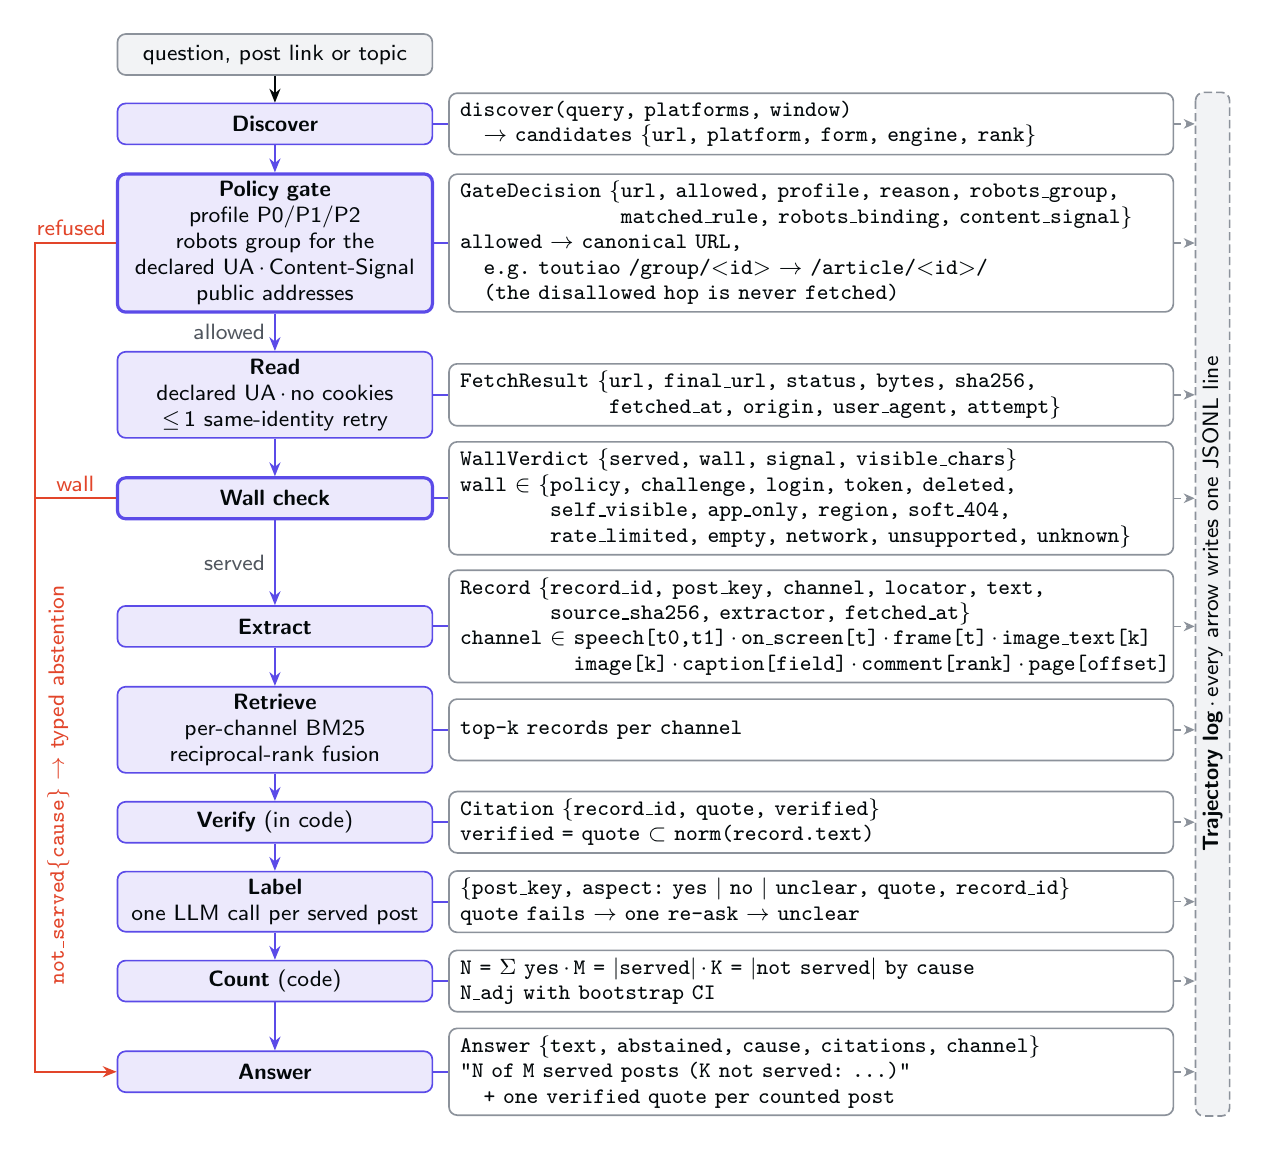
\begin{tikzpicture}[
  stage/.style={rp, text width=3.719cm, minimum height=0.52cm},
  gate/.style={rp gate, text width=3.719cm, minimum height=0.52cm},
  rec/.style={data, text width=8.919cm, minimum height=0.78cm, anchor=west},
]
\def\xs{3.05}% stage centre
\def\xd{5.25}% record west edge
% ---------------- stages ----------------
\node[neutral, text width=3.719cm, minimum height=0.52cm] (IN) at (\xs,-0.271)
  {question, post link or topic};
\node[stage] (S1) at (\xs,-1.152) {\rpt{Discover}};
\node[gate] (S2) at (\xs,-2.665) {\rpt{Policy gate}\\profile P0/P1/P2\\robots group for the\\
  declared UA\rpdot Content-Signal\\public addresses};
\node[stage] (S3) at (\xs,-4.593) {\rpt{Read}\\declared UA\rpdot no cookies\\
  $\le$\,1 same-identity retry};
\node[gate] (S4) at (\xs,-5.907) {\rpt{Wall check}};
\node[stage] (S5) at (\xs,-7.534) {\rpt{Extract}};
\node[stage] (S6) at (\xs,-8.847) {\rpt{Retrieve}\\per-channel BM25\\reciprocal-rank fusion};
\node[stage] (S7) at (\xs,-10.021) {\rpt{Verify} (in code)};
\node[stage] (S8) at (\xs,-11.030) {\rpt{Label}\\one LLM call per served post};
\node[stage] (S9) at (\xs,-12.038) {\rpt{Count} (code)};
\node[stage] (S10) at (\xs,-13.190) {\rpt{Answer}};
% ---------------- typed records ----------------
\node[rec] (D1) at (\xd,-1.152) {discover(query, platforms, window)\\
  \phantom{di}\rpto{} candidates \{url, platform, form, engine, rank\}};
\node[rec] (D2) at (\xd,-2.665) {GateDecision \{url, allowed, profile, reason, robots\_group,\\
  \phantom{GateDecision \{}matched\_rule, robots\_binding, content\_signal\}\\
  allowed \rpto{} canonical URL,\\
  \phantom{di}e.g.\ toutiao /group/\textless{}id\textgreater{} \rpto{} /article/\textless{}id\textgreater{}/\\
  \phantom{di}(the disallowed hop is never fetched)};
\node[rec] (D3) at (\xd,-4.593) {FetchResult \{url, final\_url, status, bytes, sha256,\\
  \phantom{FetchResult \{}fetched\_at, origin, user\_agent, attempt\}};
\node[rec] (D4) at (\xd,-5.907) {WallVerdict \{served, wall, signal, visible\_chars\}\\
  wall $\in$ \{policy, challenge, login, token, deleted,\\
  \phantom{wall $\in$ \{}self\_visible, app\_only, region, soft\_404,\\
  \phantom{wall $\in$ \{}rate\_limited, empty, network, unsupported, unknown\}};
\node[rec] (D5) at (\xd,-7.534) {Record \{record\_id, post\_key, channel, locator, text,\\
  \phantom{Record \{}source\_sha256, extractor, fetched\_at\}\\
  channel $\in$ speech[t0,t1]\rpdot on\_screen[t]\rpdot frame[t]\rpdot image\_text[k]\\
  \phantom{channel $\in$ }image[k]\rpdot caption[field]\rpdot comment[rank]\rpdot page[offset]};
\node[rec] (D6) at (\xd,-8.847) {top-k records per channel};
\node[rec] (D7) at (\xd,-10.021) {Citation \{record\_id, quote, verified\}\\
  verified = quote $\subset$ norm(record.text)};
\node[rec] (D8) at (\xd,-11.030) {\{post\_key, aspect:\ yes \textbar{} no \textbar{} unclear, quote, record\_id\}\\
  quote fails \rpto{} one re-ask \rpto{} unclear};
\node[rec] (D9) at (\xd,-12.038) {N = $\Sigma$ yes\rpdot M = \textbar{}served\textbar{}\rpdot
  K = \textbar{}not served\textbar{} by cause\\
  N\_adj with bootstrap CI};
\node[rec] (D10) at (\xd,-13.190) {Answer \{text, abstained, cause, citations, channel\}\\
  "N of M served posts (K not served:\ ...)"\\
  \phantom{di}+ one verified quote per counted post};
% ---------------- flow ----------------
\draw[flow] (IN) -- (S1);
\draw[rpflow] (S1) -- (S2);
\draw[rpflow] (S2) -- node[edge label, left=2pt] {allowed} (S3);
\draw[rpflow] (S3) -- (S4);
\draw[rpflow] (S4) -- node[edge label, left=2pt] {served} (S5);
\foreach \a/\b in {S5/S6,S6/S7,S7/S8,S8/S9,S9/S10}{\draw[rpflow] (\a) -- (\b);}
\foreach \i in {1,...,10}{\draw[assoc] (S\i.east) -- (D\i.west);}
% ---------------- refusal rail ----------------
\coordinate (R) at (0,0);
\draw[wallflow] (S2.west) -- (S2.west -| R) -- (S10.west -| R) -- (S10.west);
\draw[wallflow, -] (S4.west) -- (S4.west -| R);
\node[wall label, anchor=south] at ($(S2.west -| R)!0.45!(S2.west)+(0,0.04)$) {refused};
\node[wall label, anchor=south] at ($(S4.west -| R)!0.5!(S4.west)+(0,0.04)$) {wall};
\node[wall label, rotate=90] at ($(S4.west -| R)!0.5!(S10.west -| R)+(0.3,0)$)
  {{\rpmono not\_served\{cause\}} \rpto{} typed abstention};
% ---------------- trajectory log ----------------
\path let \p1=($(D1.north)-(D10.south)$) in
  node[neutral, rotate=90, minimum width=\y1, dash pattern=on 3pt off 1.5pt, anchor=north]
  (LOG) at ($(D1.north east)!0.5!(D10.south east)+(0.26,0)$)
  {\rpt{Trajectory log}\rpdot every arrow writes one JSONL line};
\foreach \i in {1,...,10}{\draw[logflow] (D\i.east) -- (D\i.east -| LOG.north);}
\end{tikzpicture}
\end{document}
